\documentclass[11pt]{article}
\usepackage[english]{babel}
\usepackage[utf8]{inputenc}
\usepackage{amsmath,amssymb,amsthm,amscd,amsfonts,amsbsy,bm}
\usepackage{listings}
\usepackage{graphicx}
\usepackage{dsfont}
\usepackage[colorinlistoftodos]{todonotes}
\usepackage{booktabs}
\usepackage{float}
\usepackage[bottom]{footmisc}
\usepackage{hyperref}
\usepackage{geometry}
\geometry{a4paper, left=1in, right=1in}
\usepackage[style=phys]{biblatex}
\addbibresource{biblio.bib}

% Misc
\DeclareMathOperator{\Max}{max}
\DeclareMathOperator{\Min}{min}
\DeclareMathOperator{\Th}{th}
\DeclareMathOperator{\Aut}{Aut}
\DeclareMathOperator{\End}{End}
\DeclareMathOperator{\Out}{Out}
\DeclareMathOperator{\interior}{Int}
\newcommand\Span[1]{\ensuremath{\langle #1 \rangle}}
\newcommand\CaptionSpace{\hspace{0.2in}}
\DeclareMathOperator{\Dim}{dim}
\newcommand\Set[2]{\ensuremath{\{\text{#1 $|$ #2}\}}}
\newcommand\Pres[2]{\ensuremath{\langle \text{$#1$ $|$ $#2$} \rangle}}
\newcommand\LPres[3]{\ensuremath{\langle \text{$#1$ $|$ $#2$ $|$ $#3$} \rangle}}
\newcommand\llangle{\ensuremath{\langle \hspace{-3pt} \langle}}
\newcommand\rrangle{\ensuremath{\rangle \hspace{-3pt} \rangle}}
\DeclareMathOperator{\Mag}{MA}

% Figures
\newcommand\Figure[4]{
\begin{figure}[t]
\centering
\centerline{\psfig{file=#2,scale=#4}}
\caption{#3}
\label{#1}
\end{figure}}

% Document specific macros go here
\newcommand\dx{\ensuremath{\text{dx}}}
\newcommand\dy{\ensuremath{\text{dy}}}
\newcommand\dz{\ensuremath{\text{dz}}}
\newcommand\df{\ensuremath{\text{df}}}
\newcommand\note[1]{\text{(#1)}}
\newcommand\mc[1]{\ensuremath{\mathcal{#1}}} % Math cal letters
\newcommand\nullset{\ensuremath{\varnothing}}
\newcommand\sfield{$\sigma$-field}
\newcommand\cyclic[1]{\ensuremath{\langle #1 \rangle}}

\newcommand{\bigslant}[2]{{\left.\raisebox{.2em}{$#1$}\middle/\raisebox{-.2em}{$#2$}\right.}}

% Nice bijection symbol
\newcommand{\bijection}{%
  \hookrightarrow\mathrel{\mspace{-15mu}}\rightarrow
}

\theoremstyle{theorem}
\newtheorem{thm}{Theorem}[section]
\newtheorem*{thm*}{Theorem}
\newtheorem{lem}[thm]{Lemma}
\newtheorem*{lem*}{Lemma}
\newtheorem{prop}[thm]{Proposition}
\newtheorem*{prop*}{Proposition}
\newtheorem{cor}[thm]{Corollary}
\newtheorem{conjecture}[thm]{Conjecture}

\theoremstyle{definition}
\newtheorem{dfn}[thm]{Definition}

\theoremstyle{remark}
\newtheorem*{rmk}{Remark}


\newcommand{\topo}[0]{\mathcal{T}}

\newcommand{\Zmod}[1]{\bigslant{\mathbb{Z}}{#1\mathbb{Z}}}
\newcommand{\F}{\ensuremath{\mathbb{F}}}
\newcommand{\norm}[1]{\left\lVert#1\right\rVert}
\newcommand{\proj}[2]{\text{proj}_{#1}{#2}}
\newcommand{\Conn}[2]{\nabla_{#1}#2}
\newcommand{\Cov}[2]{\frac{D#1}{d#2}}
\newcommand{\Pd}[1]{\partial_{#1}}
\newcommand{\InnProd}[2]{\left\langle #1, #2 \right\rangle}
\newcommand{\Lbar}[2]{\ensuremath{\overline{\mathcal{L}}(#1,#2)}}

\newcommand{\bdfn}[1][]{\ifthenelse{\equal{#1}{}}{\begin{dfn}}{\begin{dfn}[#1]}}
\newcommand{\edfn}{\end{dfn}}
\newcommand{\bthm}[1][]{\ifthenelse{\equal{#1}{}}{\begin{thm}}{\begin{thm}[#1]}}
\newcommand{\ethm}{\end{thm}}
\newcommand{\bcor}[1][]{\ifthenelse{\equal{#1}{}}{\begin{cor}}{\begin{cor}[#1]}}
\newcommand{\ecor}{\end{cor}}
\newcommand{\blem}[1][]{\ifthenelse{\equal{#1}{}}{\begin{lem}}{\begin{lem}[#1]}}
\newcommand{\elem}{\end{lem}}
\newcommand{\bprop}[1][]{\ifthenelse{\equal{#1}{}}{\begin{prop}}{\begin{prop}[#1]}}
\newcommand{\eprop}{\end{prop}}
\newcommand{\brem}{\begin{remark}}
\newcommand{\erem}{\end{remark}}
\newcommand\bpf[1][]{
\ifthenelse{\equal{#1}{}}{
\begin{proof}}
{\begin{proof}(#1)}
}
\newcommand\epf{\end{proof}}

\DeclareMathOperator*{\argmax}{arg\,max}
\newcommand\mbf[1]{\ensuremath{\mathbf{#1}}} % Math bf letters

\renewcommand{\arraystretch}{1.2}
\restylefloat{table}

\begin{document}

\begin{center}
{\LARGE Computational Physics} \\
{\Large Homework 1} \\
\vspace{4mm}
{\Large Matthew Drnevich}
\end{center}

\begin{enumerate}
\item\begin{enumerate}
    \item\begin{lstlisting}[
language=Python,
basicstyle=\scriptsize,
breaklines=true]
import numpy as np

def forward_difference(f: Callable[[np.single], np.single], x: np.single, h: np.single):
    return (f(x + h) - f(x)) / h
    
def central_difference(f: Callable[[np.single], np.single], x: np.single, h: np.single):
    two = np.single(2)
    return (f(x + h/two) - f(x - h/two)) / h
    
def extrapolated_difference(f: Callable[[np.single], np.single], x: np.single, h: np.single):
    two = np.single(2)
    eight = np.single(8)
    twelve = np.single(12)
    return (eight*f(x+h) - eight*f(x-h) + f(x - two*h) - f(x + two*h)) / (twelve*h)
\end{lstlisting}

    \item Here are the figures obtained for the error of the derivative methods.
    \begin{figure}[H]
        \centering
        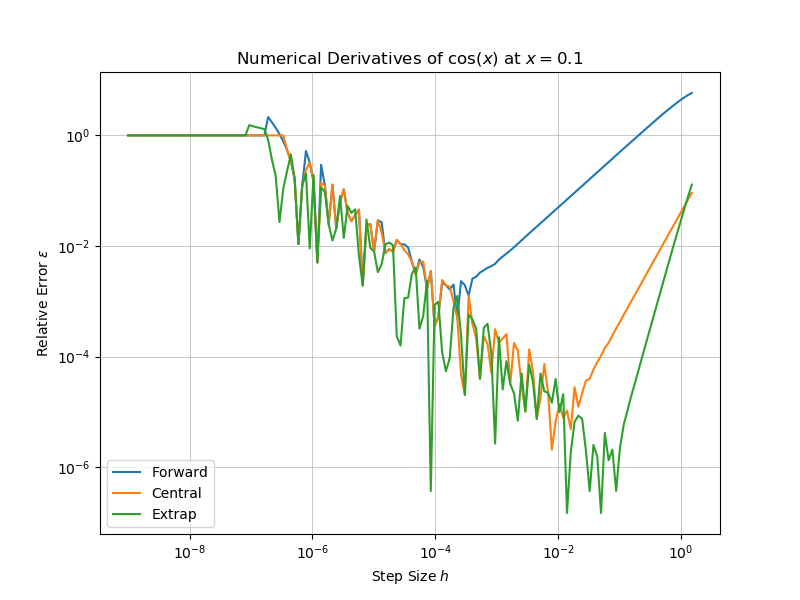
\includegraphics[scale=0.65]{derivative1.png}
        \caption{Numerical derivatives of $\cos(x)$ at $x=0.1$}
        \label{fig:my_label}
    \end{figure}
    
    \begin{figure}[H]
        \centering
        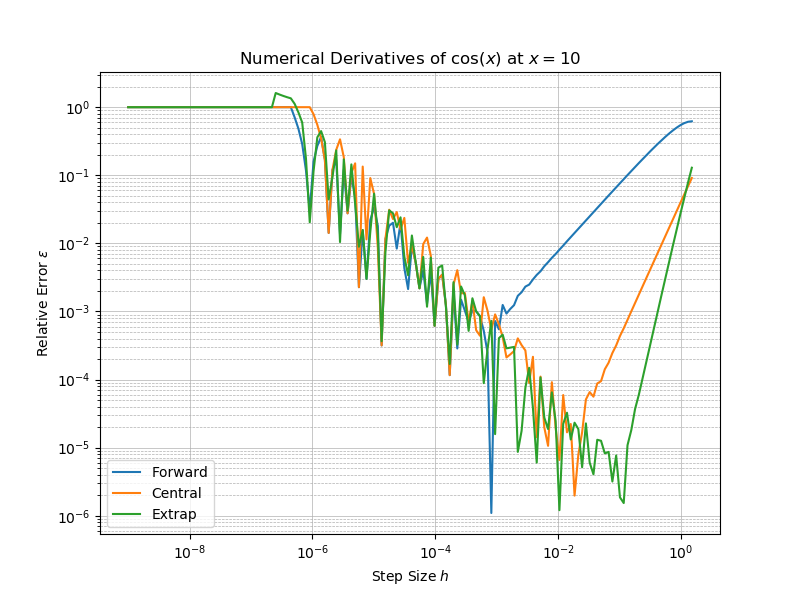
\includegraphics[scale=0.65]{derivative2.png}
        \caption{Numerical derivatives of $\cos(x)$ at $x=10$}
        \label{fig:my_label}
    \end{figure}
    
    \begin{figure}[H]
        \centering
        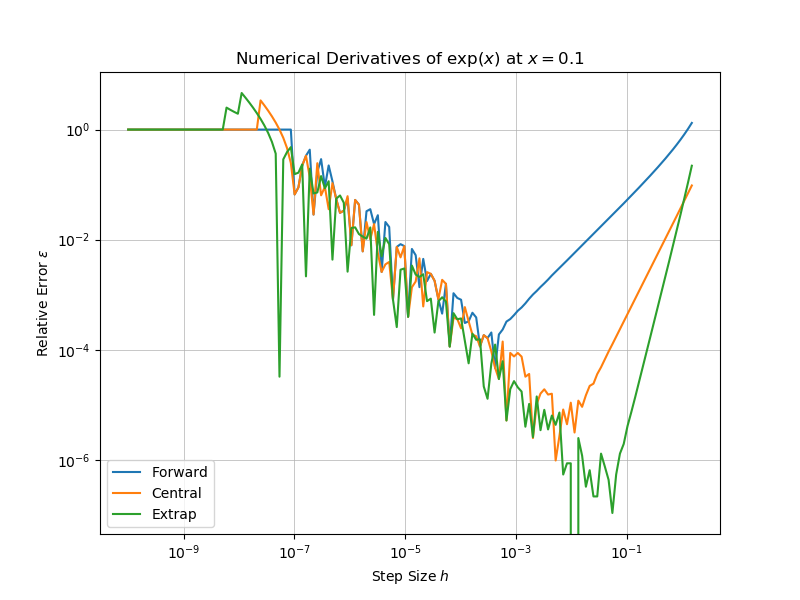
\includegraphics[scale=0.65]{derivative3.png}
        \caption{Numerical derivatives of $\exp(x)$ at $x=0.1$}
        \label{fig:my_label}
    \end{figure}
    
    \begin{figure}[H]
        \centering
        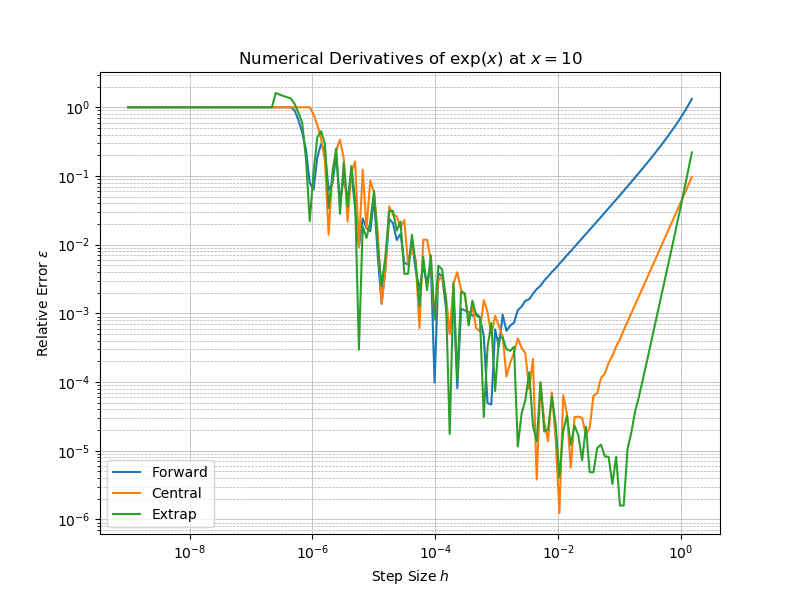
\includegraphics[scale=0.65]{derivative4.png}
        \caption{Numerical derivatives of $\exp(x)$ at $x=10$}
        \label{fig:my_label}
    \end{figure}
    
    \item At small $h$, the difference in the function values will be quite small, leading to cancellation and roundoff error, which grows with $\mathcal{O}(h^{-1/2})$, until it reaches machine precision size and gives us a derivative of zero due to roundoff error, causing the flatline. This all agrees with our graph.

    At large $h$, the approximation will be poor, leading to truncation error, which scales as
    \begin{itemize}
        \item Forward: $\mathcal{O}(h)$
        \item Central: $\mathcal{O}(h^2)$
        \item Extrapolated: $\mathcal{O}(h^4)$
    \end{itemize}
    The transition between these two errors is characterizes by the point of minimum error, i.e. the base of the ``v'' shape.
    
\end{enumerate}

\item\begin{enumerate}
    \item\begin{lstlisting}[
language=Python,
basicstyle=\scriptsize,
breaklines=true]
import numpy as np

def midpoint_rule(f: Callable[[np.single], np.single], a: np.single, b: np.single, N: np.single):
    n = int(N)
    h = (b - a) / N
    s = np.single(0)
    one = np.single(1)
    two = np.single(2)
    for k in range(n):
        s += f(a + (two*np.single(k) + one)*h/two)
    return h*s
    
def trapz_rule(f: Callable[[np.single], np.single], a: np.single, b: np.single, N: np.single):
    n = int(N)
    h = (b - a) / N
    s = np.single(0.5)*f(a) + np.single(0.5)*f(b)
    for k in range(1, n):
        s += f(a + np.single(k)*h)
    return h*s
    
def simpsons_rule(f: Callable[[np.single], np.single], a: np.single, b: np.single, N: np.single):
    n = int(N)
    h = (b - a) / N
    s = f(a) + f(b)
    two = np.single(2)
    four = np.single(4)
    for k in range(1,n,2):
        s += four*f(a + np.single(k)*h)
    for k in range(2,n,2):
        s += two*f(a + np.single(k)*h)
    return np.single(1/3)*h*s
\end{lstlisting}

    \item Here is the figure obtained for the error of the integrals.
    \begin{figure}[H]
        \centering
        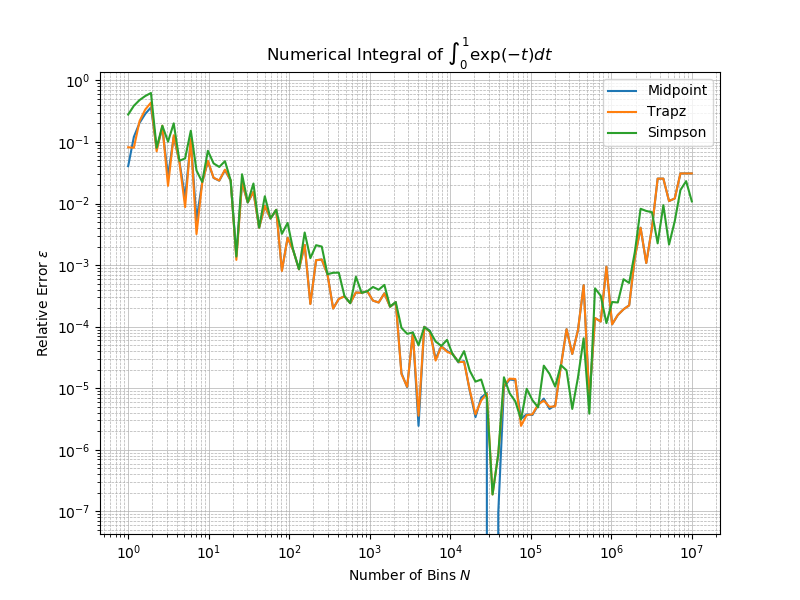
\includegraphics[scale=0.65]{integral.png}
        \caption{Numerical integral of $\int_0^1\exp(-t)dt$}
        \label{fig:my_label}
    \end{figure}
    
    \item At high $N$, the bins will be quite small, leading to small integrals, leading to roundoff error, which grows with $\mathcal{O}(\sqrt{N})$, agreeing with our graph.

    At low $N$, the approximation will be poor, leading to truncation error, which scales as
    \begin{itemize}
        \item Midoint: $\mathcal{O}(N^{-1})$
        \item Trapezoidal: $\mathcal{O}(N^{-2})$
        \item Simpson's: $\mathcal{O}(N^{-4})$
    \end{itemize}
    
    For this specific function we actually expect that each of these integration methods will roughly agree. This is because $e^{-x}$ is a monotonically decreasing function, so midpoint is a very good approximation as it's underestimates and overestimates cancel out at each step in the iteration, leaving only the endpoints for error. The same argument can be made for the trapezoidal rule. Because of this large increase in accuracies for these methods, it puts them on par with Simpson's rule for this scenario, which is why midpoint and trapezoidal rules are essentially identical in error and are very close to Simpson's.
    

\end{enumerate}

\item For this problem, first I fit a cubic spline to the given data for the function $P(k)$. Then, I used trapezoidal rule (with double precision) to evaluate $\xi(r) = \frac{1}{2\pi^2}\int_{0.0001}^{1000}dk\  k^2P(k)\frac{\sin(kr)}{kr}$. I chose the limits to be $0.0001$ and $1000$ because these were the minimum and maximum values of $k$, respectively, that were given in the datafile. If I extrapolated $P(k)$ beyond these values then my integral would be vastly incorrect, especially given the cubic spline approximation, which rapidly reaches very large negative numbers outside of this range. Therefore, the best approach given the data is to only integrate within this range. With this approach, the graph on the left shows the values of the cubic spline evaluated at the $k$ values given in the datafile, which perfectly agrees with the dataset and shows no pathological behavior. On the right, we see the resultant graph of $r^2\xi(r)$ in the range $[0,120]$ Mpc/h, which follows the shape we expected and demonstrates a BAO peak near $r = 106$ Mpc/h.
\begin{figure}[H]
    \centering
    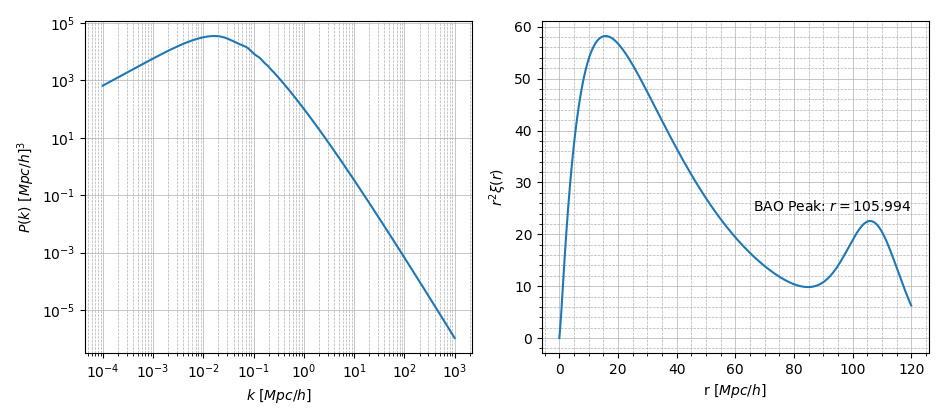
\includegraphics[scale=0.65]{problem3.png}
    \caption{Graphs demonstrating the fit of the power spectrum and the correlation function.}
    \label{fig:my_label}
\end{figure}

\end{enumerate}

\end{document}
